% !TeX root = ../build/main.tex

All the voting process is governed by the rules encoded in three smart contracts: the \textit{process management}, the \textit{sequencer registry}, and the \textit{results verification} smart contract. All these three contracts are deployed on the Ethereum blockchain, and ensure that the execution of all steps is transparent and unalterable. The protocol consists of 5 phases, as illustrated in Figure~\ref{fig:protocol-intuition}, and described below.\\

\begin{figure}[h]	
	\centerline{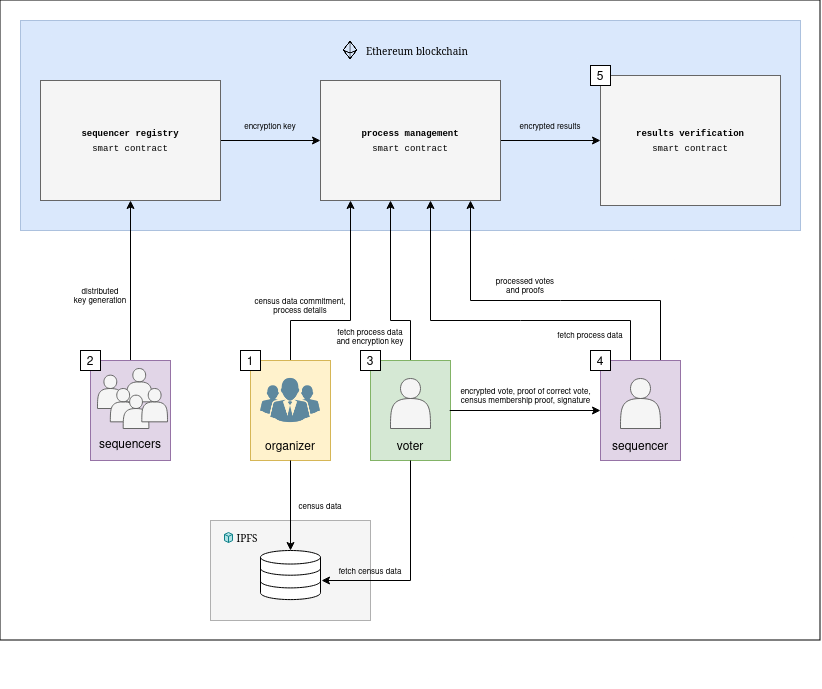
\includegraphics[width=300pt,draft=false]{\figs/protocol-intuition-flow}}
	\caption{Overview of the protocol flow.}
	\label{fig:protocol-intuition}
\end{figure}

\martai{TODO: rename the phases as they will appear in Section~\ref{sec:vocdoni-protocol}.}

\paragraph{$\boxed{1}$ Voting setup.}

In the first phase, the organizing entity gathers all census data and generates a cryptographic commitment to this data. %using a Merkle tree (MT) root. 
Additionally, the organizer defines the voting parameters, including the number of voting options and the vote-counting mechanism (e.g., weighted voting, quadratic voting, etc.). Once these details are set, the organizer submits a transaction to the process management smart contract on the Ethereum blockchain. This transaction publicly records the voting parameters and census commitment, ensuring transparency and preventing any subsequent alterations to the voting setup.

\paragraph{$\boxed{2}$ Encryption key generation.}

A designated group of participants, referred to as \textit{sequencers}, collaboratively generate a shared encryption public key, which voters will use to encrypt their votes. This key is established through a distributed key generation (DKG) protocol, ensuring that no single party can control or reconstruct the corresponding private key independently. 
Sequencers have a dual role in the protocol. In addition to generating the encryption key, they are also responsible for collecting votes from voters during the election. Consequently, their public key and the necessary information to contact them off-chain must be registered in the sequencer registry smart contract. Once the encryption public key is securely computed and published in the sequencer registry smart contract, the voting phase can start.

\paragraph{$\boxed{3}$ Voting.}

Voters select their preferred option according to the rules established by the organizer and captured in the process management smart contract. Instead of submitting their votes directly on-chain, they send them off-chain to a sequencer of their choice for processing. To ensure privacy, votes are encrypted using the available encryption public key. Alongside the encrypted vote, each voter must also provide the following data: a proof of valid voting, demonstrating that the vote complies with the election rules; a proof of eligibility, verifying that they are registered in the census; and a proof of identity ownership, in the form of a digital signature, confirming that they are the legitimate voter and are not impersonating someone else. 
\martai{In the above paragraph, we could include a short description about double-voting/overwriting: add the goal/idea of the commitment and the nullifier.}

\paragraph{$\boxed{4}$ Votes collection.}

During this phase, sequencers collect encrypted votes from multiple voters along with their corresponding proofs, and verify the validity of these submissions. That is, sequencers
verify the signatures, to ensure the votes were cast by legitimate voters, they verify the proof of compliance, confirming that each vote adheres to the polling rules, and the census membership proofs against the commitment to the census data that was originally registered in the process management smart contract. Once the sequencers have processed and verified all votes, they must prove that these verifications were performed correctly. Instead of submitting individual verifications for each vote, they generate a single zero-knowledge (ZK) proof that attests to the correctness of all verifications.
%they compress multiple individual verification into one.
Additionally, the sequencers reencrypt the votes and generate a proof of the correct reencryption computation. While this process does not alter the final tally, it prevents voters from decrypting their original vote. This step mitigates vote selling or coercion, as voters are no longer able to prove their choice to third parties. Finally, the sequencers submit the reencrypted votes along with their verification and reencryption proofs to the process management smart contract. The smart contract verifies all the proofs provided by the sequencers to check that they complied with the protocol.

\paragraph{$\boxed{5}$ Results verification.}

\martai{I did not look into the results decryption/verification part yet. A short description should be given here.}

\textit{Old text: At the conclusion of the voting period, the smart contract ceases to accept new state updates, effectively finalizing the process. The final State is then available on-chain for verification, providing an immutable record of the voting outcome.}